\documentclass{ethz_report}
\usepackage{listings}
\usepackage{color}
\usepackage{caption}
\usepackage{subcaption}


\definecolor{codegreen}{rgb}{0,0.6,0}
\definecolor{codegray}{rgb}{0.5,0.5,0.5}
\definecolor{codepurple}{rgb}{0.58,0,0.82}
\definecolor{backcolour}{rgb}{1,1,1}

\lstdefinestyle{mystyle}{
    backgroundcolor=\color{backcolour},
    commentstyle=\color{codegreen},
    keywordstyle=\color{magenta},
    numberstyle=\tiny\color{codegray},
    stringstyle=\color{codepurple},
    basicstyle=\ttfamily,
    breakatwhitespace=false,
    breaklines=true,
    captionpos=b,
    keepspaces=true,
    numbers=left,
    numbersep=5pt,
    showspaces=false,
    showstringspaces=false,
    showtabs=false,
    tabsize=4,
    frame=lines
}
\lstset{style=mystyle}

\title{Exercise 4 - Model Fitting}
\subject{Computer Vision}
\author{Alberto Montes}
\email{malberto@student.ethz.ch}
\date{\today}

\begin{document}
\maketitle

\section*{Line Fitting with RANSAC}

For the first exercise which consist to code the RANSAC algorithm for line fitting. The algorithm
follows the guidelines of its design, which iterating over a fixed number of times, two points are
randomly chosen, fit a line on it and compute the inline and outlines points. If there is enough
inline points, the line is refitted for all this points and the one with the best inline ratio is
kept to be returned. The code is on the attached code and the results obtained with the
examples cloud point are on Figure~\ref{fig:ransac_img}. As the algorithm was design to be less sensitive
to outliers, at the results can be seen how the predicted line by the algorithm is almost the same
as the original one.

%\lstinputlisting[language=MATLAB, caption=ransacLine.m, label={lst:ransac}]{../code/ransacLine.m}

\begin{figure}[H]
\centering
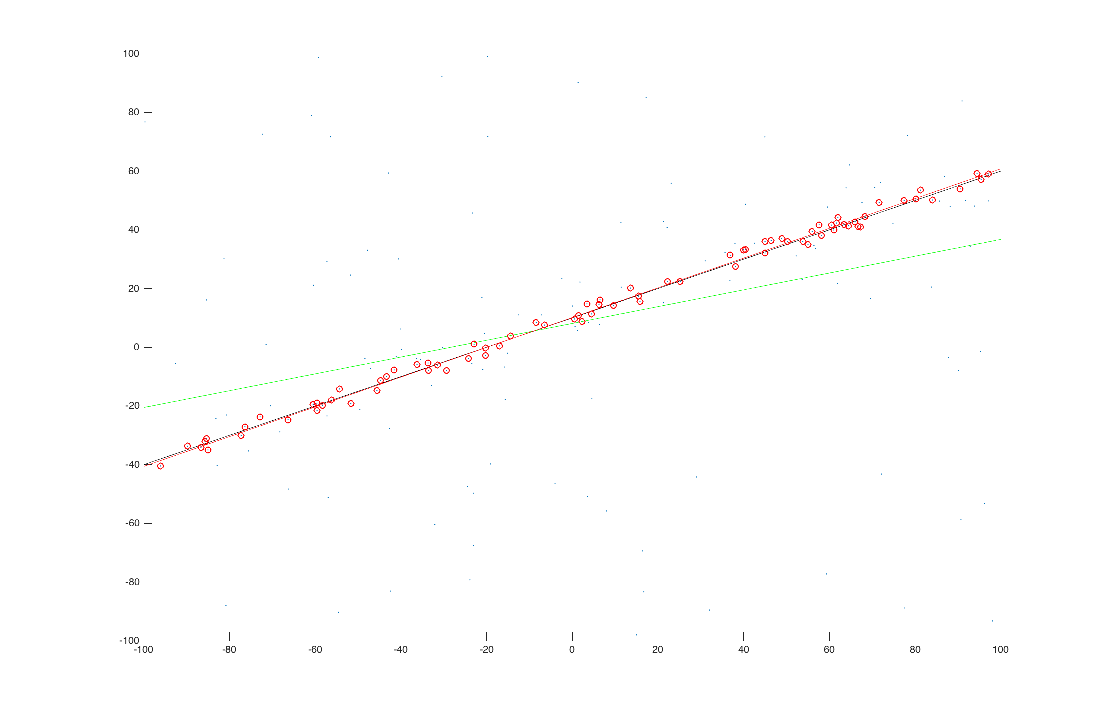
\includegraphics[width=.8\linewidth]{images/ransac.png}
\caption{Results of line fitting using RANSAC algorithm.}
\label{fig:ransac_img}
\end{figure}

\section*{Fundamental Matrix}

The next exercise consist on finding the fundamental matrix from the given points of two different
images from the same scenario. The implemented code can be found in the Listing~\ref{lst:fundamental_matrix}.

\lstinputlisting[language=MATLAB, caption=fundamentalMatrix.m, label={lst:fundamental_matrix}]{../code/fundamentalMatrix.m}

The implementation first normalize all the given points. Then with the eight-point algorithm find
the values of the non-singular fundamental matrix $F$, and then, enforcing the singularity
constrain, finds the fundamental matrix $\hat F$. Once is computed the fundamental matrix, the
epipolar lines can be drawn from one image point to the other one, an on Figure~\ref{fig:fun_mat}
there is the result.

\begin{figure}[H]
\centering
\begin{subfigure}[b]{.5\textwidth}
  \centering
  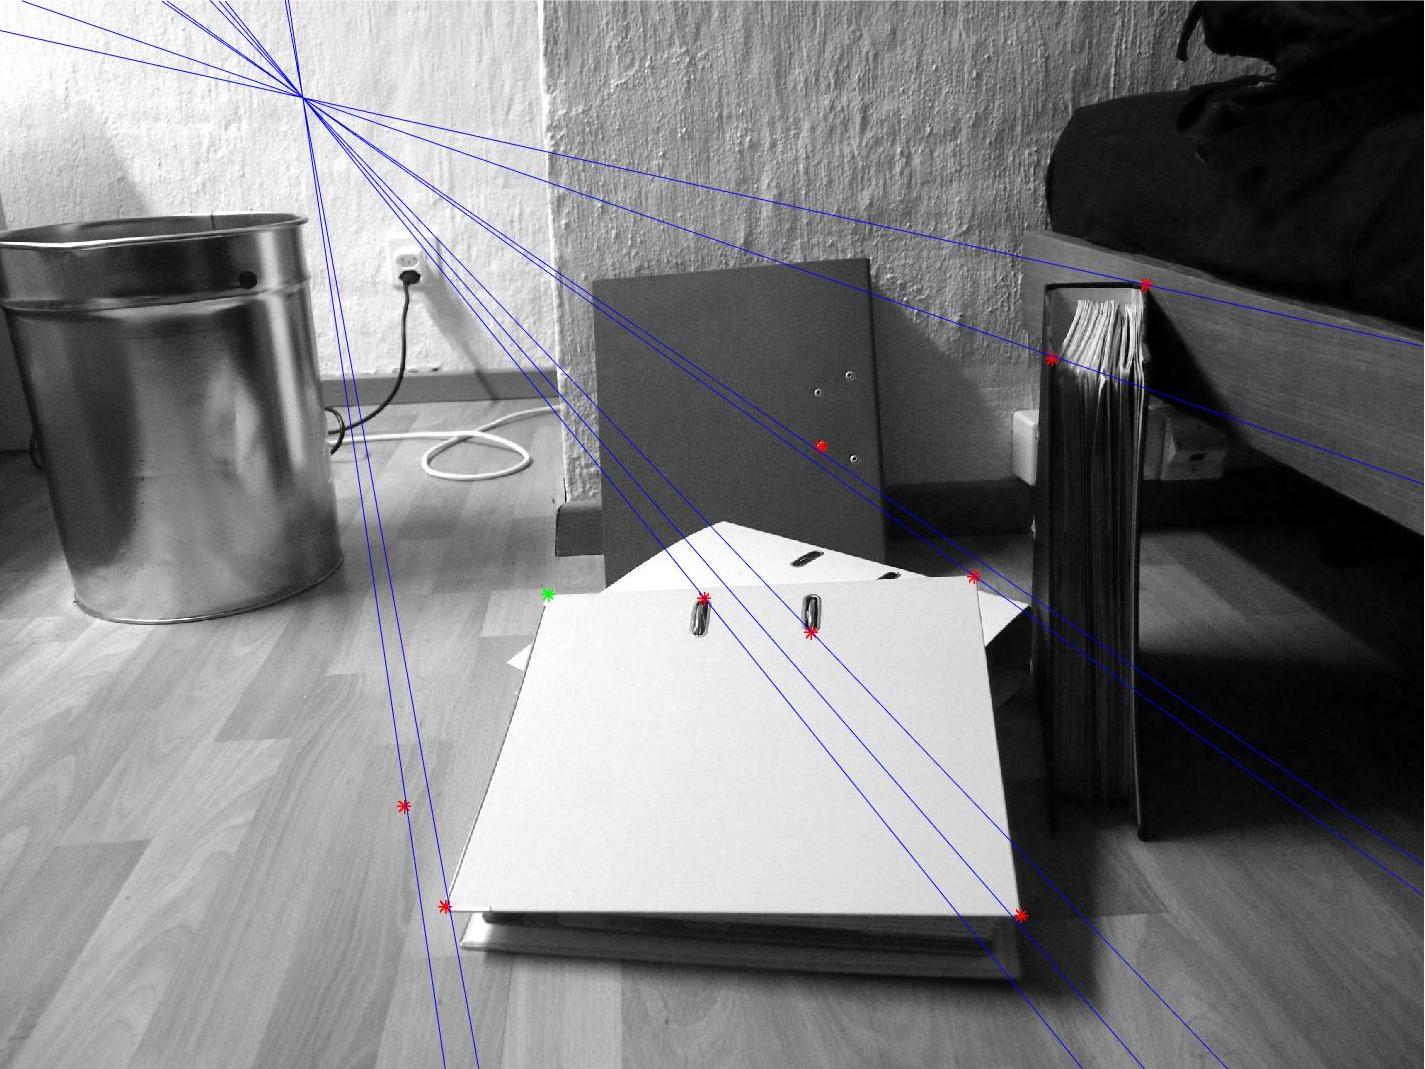
\includegraphics[width=1\linewidth]{images/fmatrix_1}
\end{subfigure}%
\begin{subfigure}[b]{.5\textwidth}
  \centering
  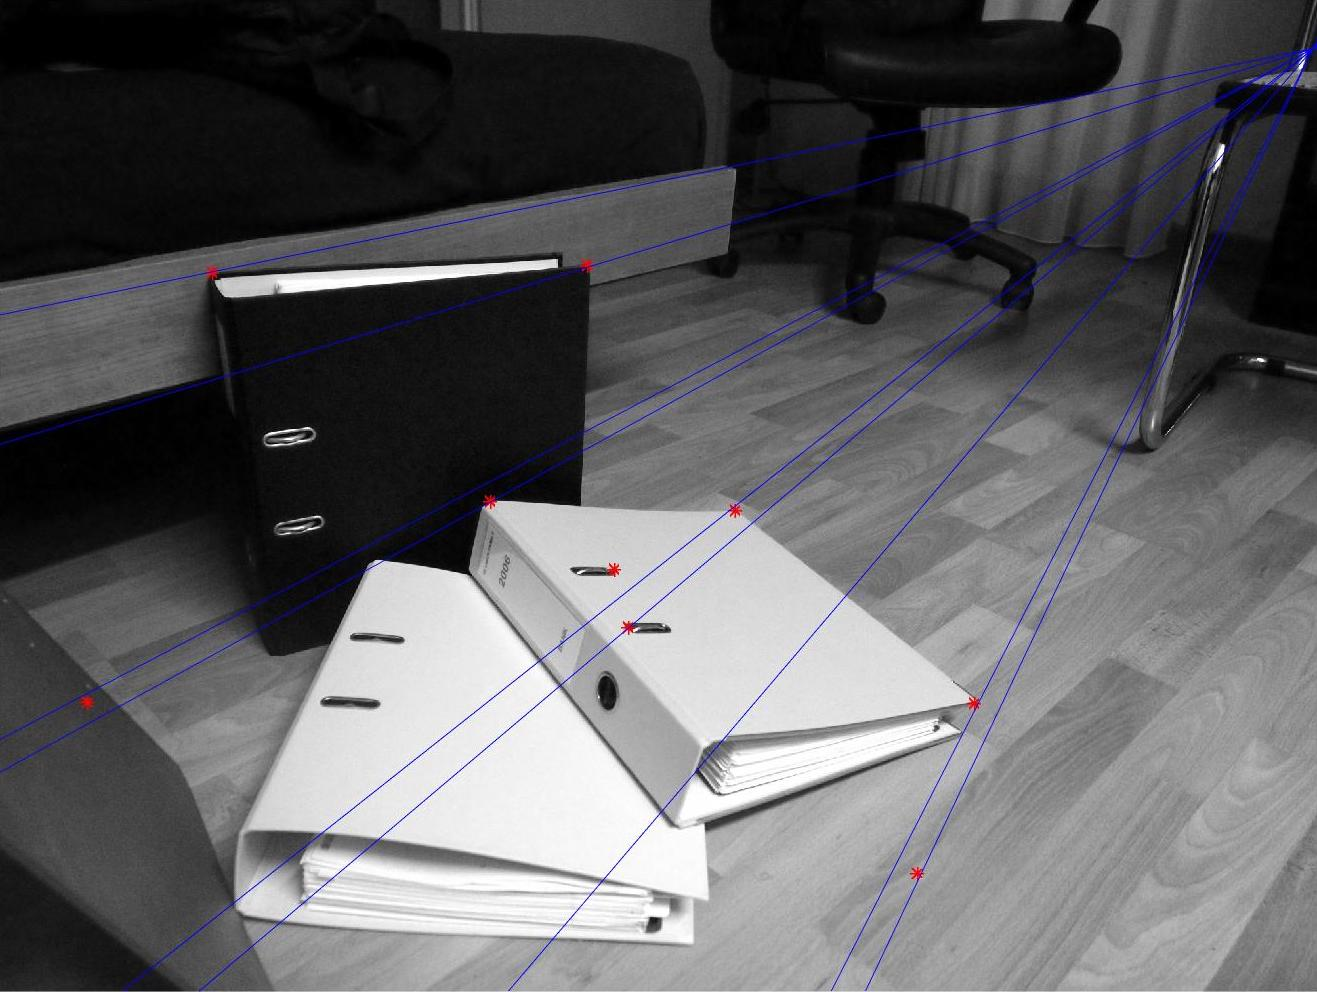
\includegraphics[width=1\linewidth]{images/fmatrix_2}
\end{subfigure}
\caption{Epipolar lines obtained with the Fundamental Matrix $\hat F$.}
\label{fig:fun_mat}
\end{figure}

\section*{Essential Matrix}

The next step, has been to compute the Essential Matrix from the normalized points using the camera
matrix. The way to compute it is the same as the eight-point algorithm previously used with the
fundamental matrix. To take into account, it has been enforced the restriction to Essential Matrix
to have the same value at the first two singular values. The implementation is on
Listing~\ref{lst:essential_matrix} and the epipolar lines drawn from the computed essential matrix
is plot on Figure~\ref{fig:es_mat}.

\lstinputlisting[language=MATLAB, caption=essentialMatrix.m, label={lst:essential_matrix}]{../code/essentialMatrix.m}

\begin{figure}[H]
\centering
\begin{subfigure}[b]{.5\textwidth}
  \centering
  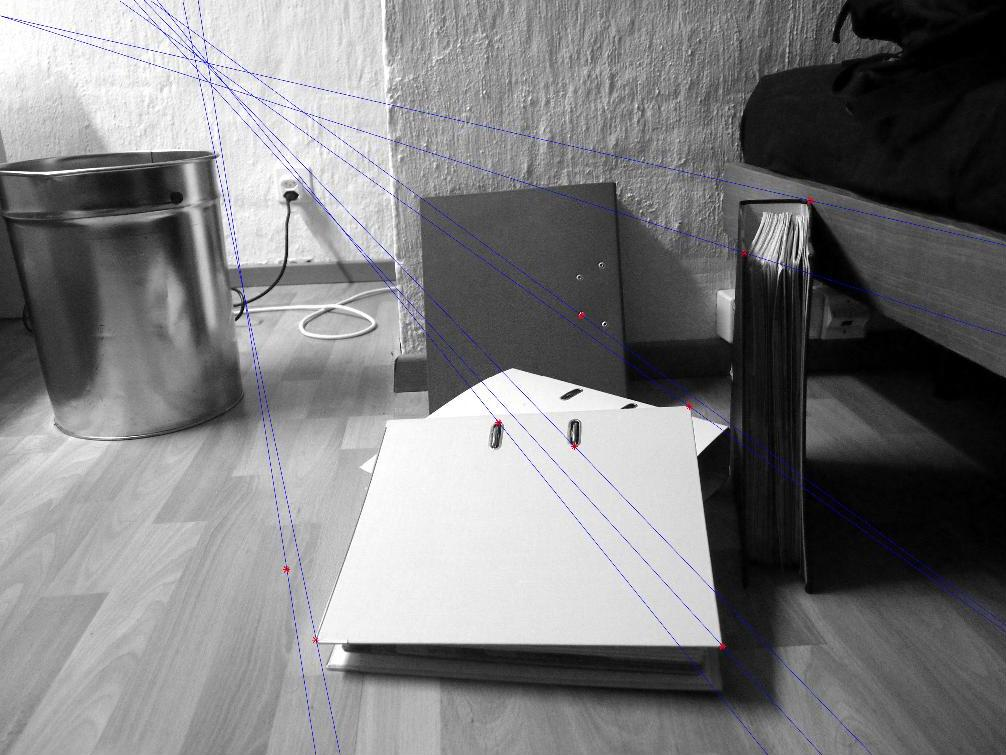
\includegraphics[width=1\linewidth]{images/ematrix_1}
\end{subfigure}%
\begin{subfigure}[b]{.5\textwidth}
  \centering
  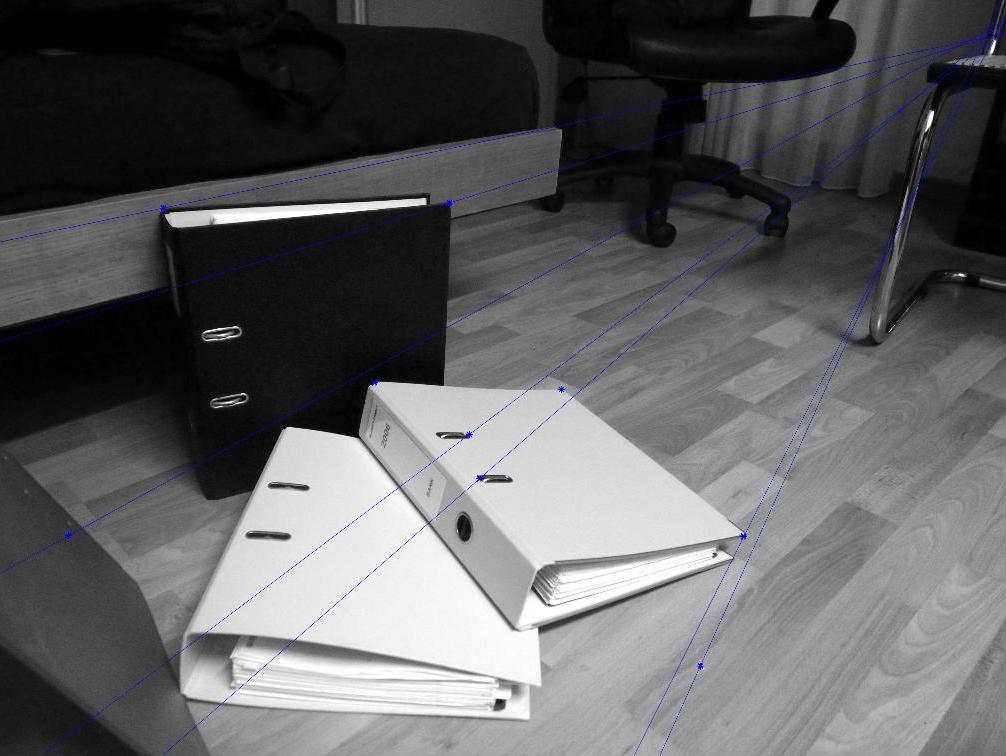
\includegraphics[width=1\linewidth]{images/ematrix_2}
\end{subfigure}
\caption{Epipolar lines obtained with the Essential Matrix $E$.}
\label{fig:es_mat}
\end{figure}

\section*{Camera Matrix}

To compute the camera matrix $P'$, it has been necessary to compute decompose the Essential Matrix
into $R$ and $t$ and find the better combination of both (two possible directions and two possible
rotations). To do so, it has been computed the four combinations, and then chose the one which the
projected coordinates are placed in front of the camera, so the $z$ coordinate is positive for all
the available points (the 3D points representation is on Figure~\ref{fig:3d_points}). On Listing~\ref{lst:decompose_E} is the implementation to decompose the
Essential Matrix. In addition I would like to remark that it is important to ensure that the
$det(R) = 1$ in positive sign.

\lstinputlisting[language=MATLAB, caption=decomposeE.m, label={lst:decompose_E}]{../code/decomposeE.m}

\begin{figure}[H]
\centering
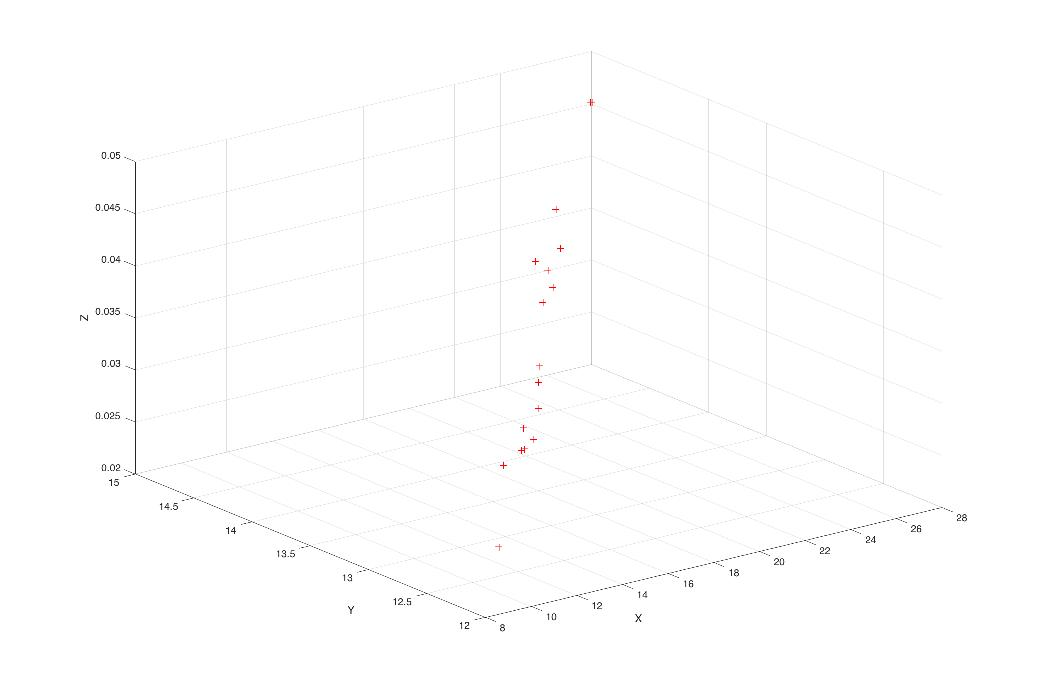
\includegraphics[width=.7\linewidth]{images/3d_essential_m}
\caption{3D points representation.}
\label{fig:3d_points}
\end{figure}

\section*{Feature Extraction and Matching}

To perform a feature matching, it has been computed the SIFT features using the VLEAF implementation
and then plot the matching in both formats: side by side as in Figure~\ref{fig:features_matching}
and overlap as in Figure~\ref{fig:features_matching_overlap}.

\begin{figure}[H]
\centering
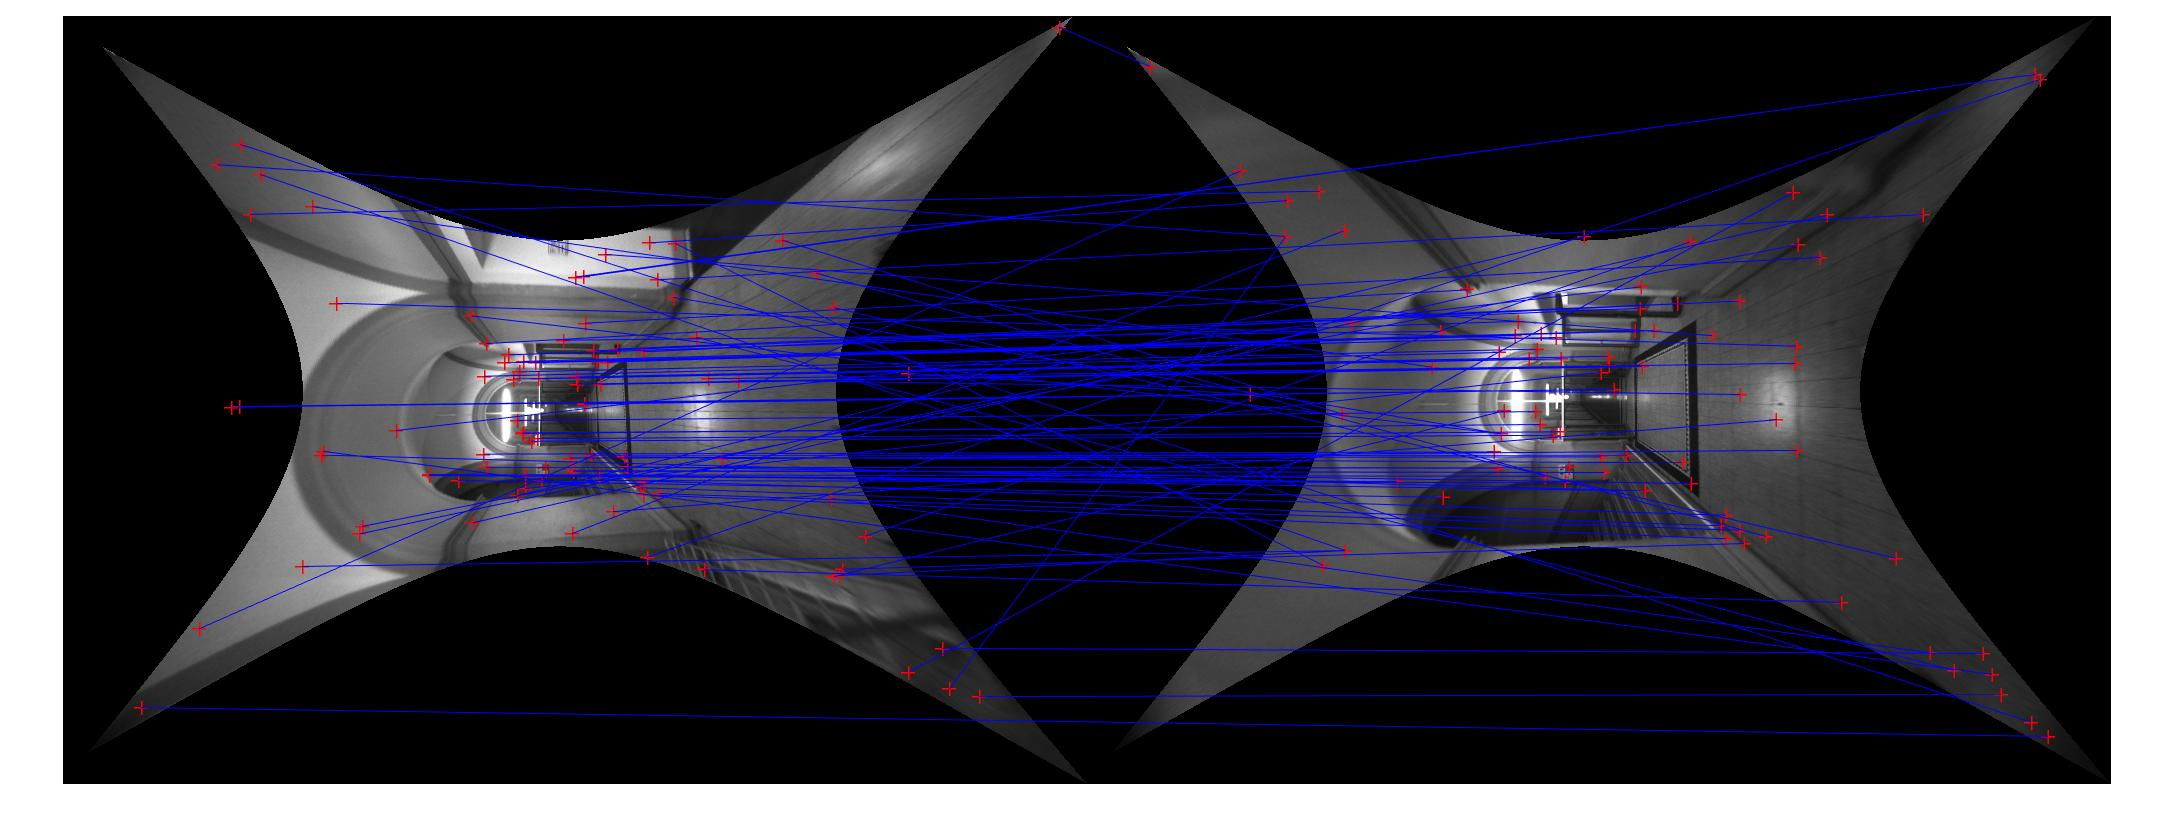
\includegraphics[width=1\linewidth]{images/sift_matching}
\caption{SIFT Features matching.}
\label{fig:features_matching}
\end{figure}

\begin{figure}[H]
\centering
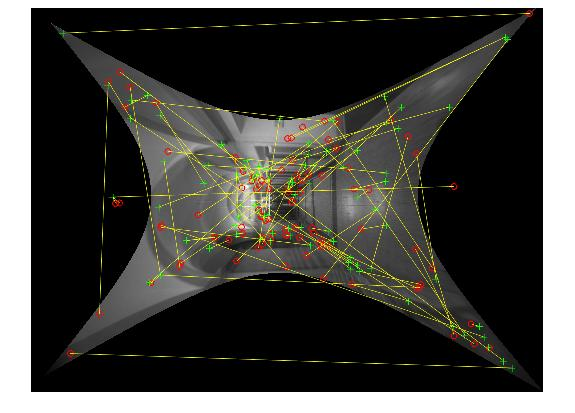
\includegraphics[width=.8\linewidth]{images/sift_matching_2}
\caption{SIFT Features matching (overlap).}
\label{fig:features_matching_overlap}
\end{figure}

\section*{8-Point RANSAC}

Finally, the 8-point RANSAC algorithm has been used to find the fundamental matrix and improve the
features matching seen in Figure~\ref{fig:features_matching}. The algorithm is the same as in
implemented at the beginning, but in this case, the fundamental matrix is computed and the distance
is the computation of the distance of the correspondence point to the epipolar line.

On Listing~\ref{lst:ransac8pF} there is the implementation of the algorithm. Also, in addition, on
Figure~\ref{fig:features_matching_ransac} there is plot the inliears matchings as green and the
outliers matchings as red.

\lstinputlisting[language=MATLAB, caption=ransac8pF.m, label={lst:ransac8pF}]{../code/ransac8pF.m}

\begin{figure}[H]
\centering
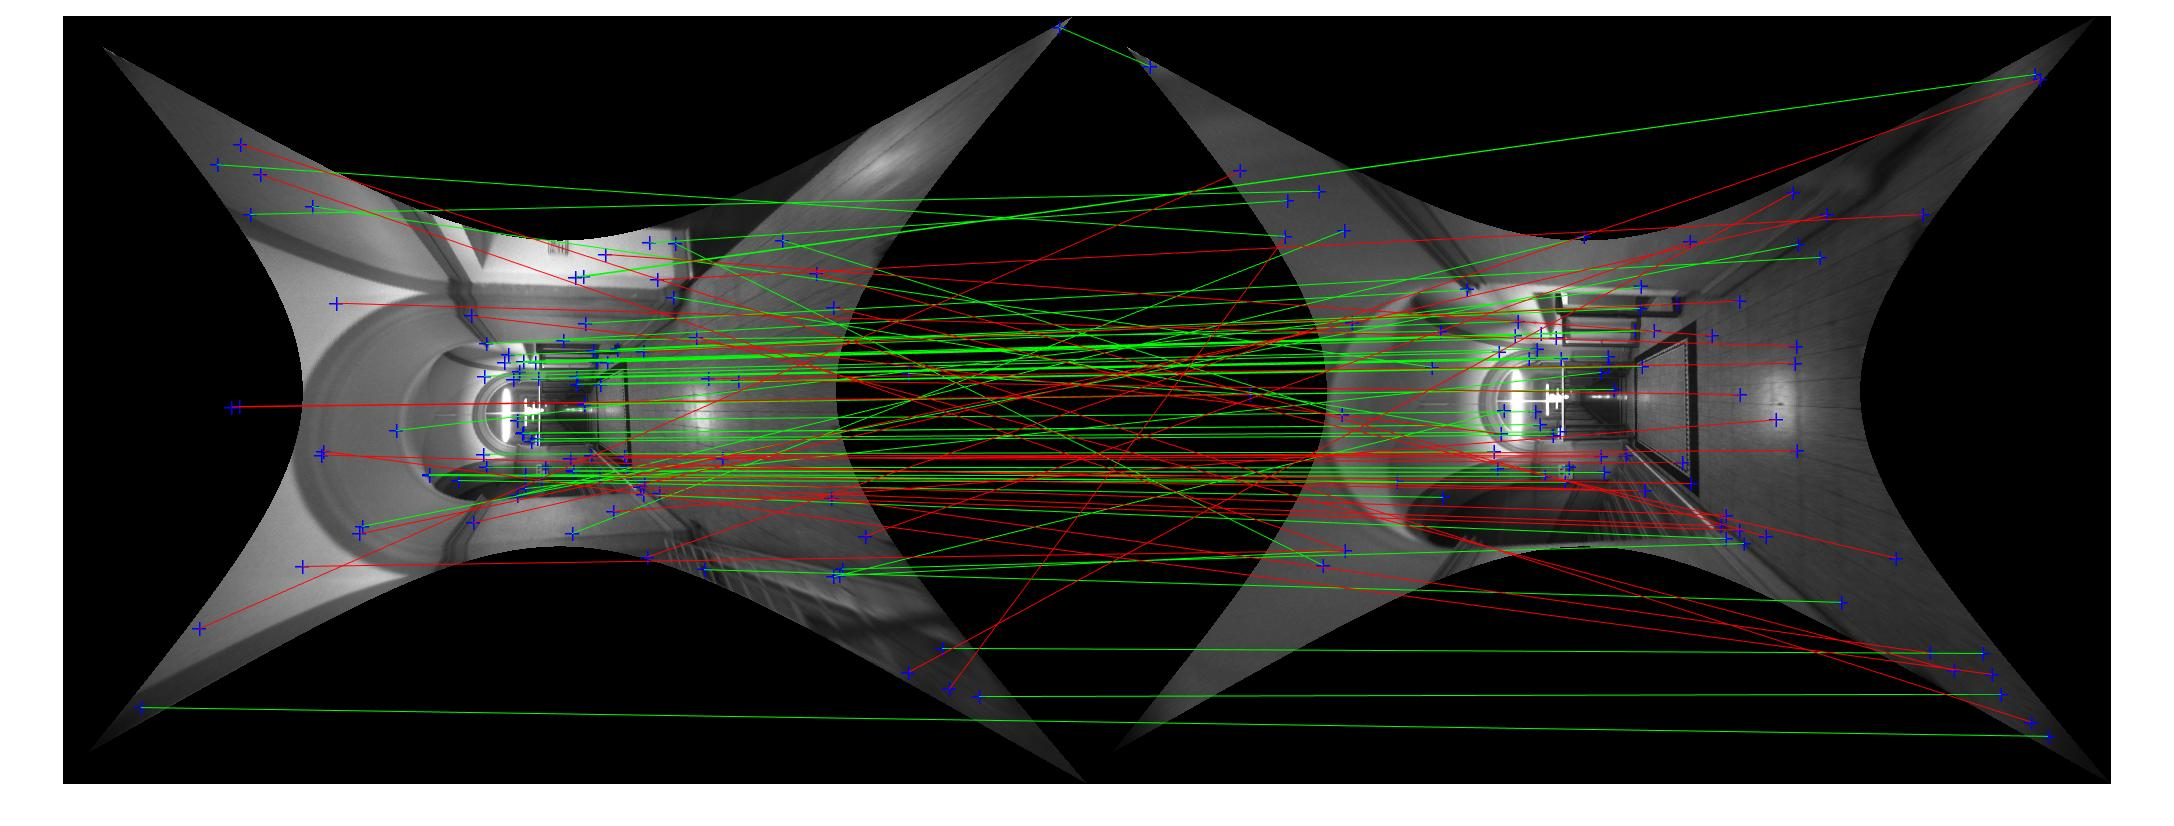
\includegraphics[width=1\linewidth]{images/ransac8p_features}
\caption{Features matching using the 8-point RANSAC algorithm for Fundamental Matrix}
\label{fig:features_matching_ransac}
\end{figure}

\end{document}
